\documentclass[12pt]{article}
\usepackage{graphicx,url}
\usepackage[brazil]{babel}
\usepackage[utf8]{inputenc}
\usepackage{array,amsmath,booktabs}
\usepackage[table,xcdraw]{xcolor}
\usepackage{amsmath}
\usepackage[portuguese,ruled,lined]{algorithm2e}
\usepackage{algorithmic}
\usepackage{xcolor}
\definecolor{verde}{rgb}{0,0.5,0}
\usepackage{listings}
\lstset{
  language=C++,
  basicstyle=\ttfamily\small, 
  keywordstyle=\color{blue}, 
  stringstyle=\color{verde}, 
  commentstyle=\color{red}, 
  extendedchars=true, 
  showspaces=false, 
  showstringspaces=false, 
  numbers=left,
  numberstyle=\tiny,
  breaklines=true, 
  backgroundcolor=\color{white!10},
  breakautoindent=true, 
  captionpos=b,
  xleftmargin=0pt,
}
\newcommand\tab[1][1cm]{\hspace*{#1}}
\title{Força Bruta, Programação Dinâmica e Algoritmos Gulosos\\URI: Troco(2446)}
\author{Luiz Fellipe Machi Pereira(RA 103491)\\Diogo Fernando de Melo Sales(RA 93814)}
\begin{document} 

\maketitle

\section{Descrição do Problema}

Você está num supermercado e está na fila do caixa para comprar alguns produtos. Assim que você termina de passar as compras pelo caixa, se lembra que tem várias moedas em seu bolso, algumas repetidas, e fica pensando se com elas dá para pagar exatamente o valor das compras (para assim se livrar destas moedas e ficar com os bolsos mais leves). Você consegue pagar o valor exato da conta usando estas moedas?
\subsection{Entrada}
A primeira linha da entrada contém dois números inteiros \textbf{V} $(1 \leq V \leq 10^{5})$ e \textbf{M} $(1 \leq M \leq 10^{3})$, indicando, respectivamente, o valor final da compra e o número de moedas que você tem em seu bolso. A segunda linha contém M números inteiros que descrevem o valor \textbf{M}{i} $(1 \leq M{i} \leq 10^{5})$ de cada moeda existente em seu bolso.
\subsection{Saída}
Seu programa deve imprimir apenas uma linha, contendo apenas um caractere: S caso seja possível pagar o valor exato da conta usando apenas suas moedas, ou N caso contrário.
\section{Formulação recursiva}
$opt(m,V) = \left \{ \begin{matrix} True & \mbox{se }V\mbox{$= 0$} \\ False & \mbox{se }m < 0\mbox{  e V} > 0 \\ opt(m-1,V - M[m])   
\\\vee \; opt(m-1,V) & \mbox{se }M \geq 0\mbox{  e V} > 0 \end{matrix} \right.$
\section{Substrutura ótima}
Para mostrar que há subestrutura ótima devemos analisar dois casos:\\
\textbf{A)} $m \in S$ (Considere agora que o valor $M[m]$ faça parte da solução ótima). Assumimos que $S^{*} = opt(m-1,V - M[m]) \cup M[M]$ onde $m$ é quantidade de moedas que você tem no bolso, $V$ é o valor final da compra e o vetor $M$ representa o valor de cada moeda, é a solução ótima para o problema de tamanho $m$. Suponha que exista outra solução $A^{*} = opt'(m-1,V -M[m])$ que devolve um valor estritamente menor do que $S^{*} - M[m]$, ou seja, exista uma forma de obter o valor $V$ utilizando menos moedas e que devolve $Verdadeiro$. Portanto, há como melhorar a solução ótima utilizando $A^{*}\cup M[m]$, o que é uma contradição.\\ 
\textbf{B)} $m \in S = S$ e $M[m]$ não faz parte da solução ótima então $S = [1...m-1]$ tem que ser a solução ótima para o subproblema. A prova é análoga ao caso anterior.
\section{Sobreposição de problemas}
Para demonstrar que o problema apresenta sobreposição de problemas foi usado o método de árvore de recursão Figura \ref{fig:arvore}.
\begin{figure}[h]
\centering
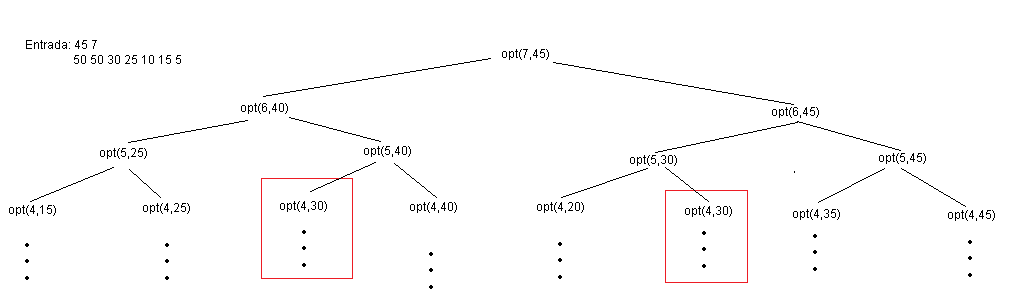
\includegraphics[width=.9\textwidth]{arvore.png}
\caption{Árvore de Recursão\label{fig:arvore}}
\end{figure}
\section{Análise de Complexidade}
\subsection{Força Bruta}
A recorrência força bruta T(V) é dada pelo seguinte somatório, onde $V$ é o valor do troco, $m$ é quantidade de moedas disponíveis indo de [$M[1]$...$M[m]$] e $M[i]$ é o valor de cada moeda. Para determinar sua complexidade mais precisamente é necessário encontrar uma fórmula fechada para o somatório das recorrências abaixo.\\
$\displaystyle\sum_{i=0}^{m} T(V - M[i])$
\subsection{Programação dinâmica/memoizado}
Para determinar qualquer complexidade de um algoritmo memoizado, é necessário fazer o cálculo do Número de subproblemas distintos vezes o Custo de cada subproblema, em nosso caso, a quantidade de subproblemas é $(m \ldotp V)$ (memo), onde $m$ é a quantidade de moedas disponíveis e $V$ o valor desejado, e o custo de cada linha é constante, visto que as chamadas recursivas têm custo constante e as comparações também. Portanto a complexidade do algoritmo é $O(m \ldotp V)$.
\section{Escolha Gulosa}
Nossa proposta de algoritmo guloso é ordenar o vetor de moedas, percorrer o vetor em busca de encontrar uma moeda de valor igual a $V$, caso não exista, o algoritmo pega as menores moedas e vai somando, se a soma for igual a $V$ o algoritmo retorna $Verdadeiro$, se a soma for maior que $V$ retorna-se $Falso$. O algoritmo falha quando a única solução é um valor grande de uma moeda somado com um valor pequeno de moeda.
\begin{lstlisting}
def troco(coins,qtd,val):
	soma = 0
	for i in range(len(coins)):
		if soma == val:
			return True			
		elif soma > val:
			return False
		else:
			soma += coins[i]						

val = [int(i) for i in input().split()]
v = val[0]
m = val[1]
coins = [int(i) for i in input().split()]
coins.sort()
for x in range(len(coins)):
	if coins[x] == v:
		flag = 1
		break
if flag == 1:
	print('S')
else:
	if troco(coins,m-1,v) == True:
		print('S')
	else:
		print('N')

\end{lstlisting} 

\section{Casos de teste} \label{sec:marker}
$Entrada\;1: \left \{ \begin{matrix} 16\;4 & \mbox{}\mbox{}\\
25\;10\;5\;1 & \mbox{}\mbox{}\end{matrix} \right.$
\\
\tab Saída 1: S\\
$Entrada\;2: \left \{ \begin{matrix} 20\;4 & \mbox{}\mbox{}\\
25\;10\;5\;1 & \mbox{}\mbox{}\end{matrix} \right.$
\\
\tab Saída 2: N\\
$Entrada\;3: \left \{ \begin{matrix} 35\;10 & \mbox{}\mbox{}\\
33\;33\;32\;31\;30\;25\;20\;14\;7\;1 & \mbox{}\mbox{}\end{matrix} \right.$
\\
\tab Saída 3: S\\
$Entrada\;4: \left \{ \begin{matrix} 21\;4 & \mbox{}\mbox{}\\
25\;10\;5\;1 & \mbox{}\mbox{}\end{matrix} \right.$
\\
\tab Saída 4: N\\
$Entrada\;5: \left \{ \begin{matrix} 9270\;20 & \mbox{}\mbox{}\\
269\;657\;124\;367\;150\;961\;290\;856\;304\;929\;665\;231\;877\;377\;447\;965\;82\;661\;462\;617 & \mbox{}\mbox{}\end{matrix} \right.$
\\
\tab Saída 5: S
\section{Comparação de algorítimos}
Para efetivar a melhora trazida pela PD foram comparadas as versões em modo Força Bruta, Memoizado e Iterativo do problema Troco(2446). A tabela a seguir apresenta os resultados Tabela \ref{tab:comp}. 
\begin{table}[h]
\centering
\caption{Comparação dos Algoritmos no quesito tempo.}
\label{tab:comp}
\begin{tabular}{|l|l|l|l|}
\hline
\rowcolor[HTML]{FFCC67} 
Tipo & Força Bruta & Memoizado & \cellcolor[HTML]{FFCB2F}Iterativo \\ \hline
Real & 0,039s      & 0,039s    & 0,005s                            \\ \hline
User & 0,026s      & 0,032s    & 0,000s                            \\ \hline
Sys  & 0,013s      & 0,007s    & 0,005s                            \\ \hline
\end{tabular}
\end{table}

 No caso para todos os algoritmos foi usada a Entrada 1 especificada na sessão \ref{sec:marker}.
\begin{description}
\item{\textbf{Força Bruta}}\begin{lstlisting}
def troco(coins,qtd,val):
	if val >= 0 and qtd >= 0:
		if val == 0:
			return True
		elif(qtd < 0 and val > 0):
			return False
		else:
			return troco(coins,qtd-1,val - coins[qtd]) or troco(coins,qtd-1,val)
	else:
		return False

val = [int(i) for i in input().split()]
v = val[0]
m = val[1]
coins = [int(i) for i in input().split()]
if troco(coins,m-1,v) == True:
	print('S')
else:
	print('N') 
    
    \end{lstlisting} 
 \item{\textbf{Memoizado}}
 \begin{lstlisting}
def troco(coins,qtd,val,memo):
	if qtd < 0 or val <0:
		return False
	else:
		if memo[qtd][val] == -1:
			if val == 0:
				ans = True
			elif(qtd < 0 and val > 0):
				ans = False
			else:
				ans = troco(coins,qtd-1,val - coins[qtd],memo) or
                	troco(coins,qtd-1,val,memo)
				memo[qtd][val] = ans
	return memo[qtd][val]

val0 = [int(i) for i in input().split()]
v = val0[0]
m = val0[1]
coins = [int(i) for i in input().split()]
memo = []
for x in range(m+1):
	lines = []
	for x in range(v+1):
		lines.append(-1)
	memo.append(lines)
	
if troco(coins,m-1,v,memo) == True:
	print('S')
else:
	print('N')
    
    \end{lstlisting}
 
 \item{\textbf{Iterativo}}
 
  \begin{lstlisting}
#include <iostream>

using namespace std;

int troco(int coins[], int m, int v){
	int ans,memo[m+1][v+1];

	for (int i = 0; i <= m; ++i){
		memo[i][0] = 1;
	}
	for (int i = 1; i <= v; ++i){
		memo[0][i] = 0;
	}
	for (int i = 1; i <= m; i++){
		for (int j = 1; j <= v; j++){
			if (j < coins[i-1]){
				memo[i][j] = memo[i-1][j];
			}
			else{
				memo[i][j] = memo[i-1][j] || memo[i-1][j-coins[i-1]];
			}
		}
	}
	return memo[m][v];
}

int main(){
	int v = 0,m = 0,s=0;
	cin >> v >> m;
	int coins[m];

	for (s = 0; s < m; s++){
		cin >>coins[s];
	}

	if (troco(coins,m,v) == 1){
		printf("S\n");
	}else{
		printf("N\n");
	}
}
    
    \end{lstlisting}

 \end{description}

\section{Referências}
O PROBLEMA subset-sum. Disponível em: \url{https://www.ime.usp.br/~pf/analise_de_algoritmos/aulas/mochila-subsetsum.html}. Acesso em: 23 jun. 2018.\\
DYNAMIC Programming | Set 25 (Subset Sum Problem). Disponível em: \url{https://www.geeksforgeeks.org/dynamic-programming-subset-sum-problem/}. Acesso em: 23 jun. 2018.\\
URI Online Judge | 2446. Disponível em: \url{https://www.urionlinejudge.com.br/judge/pt/problems/view/2446}. Acesso em: 23 jun. 2018.
\end{document}
